%\documentclass[12pt]{report}
%\documentclass[12pt]{extreport}
\documentclass[17pt]{extarticle}
%\documentclass{memoir}

\usepackage{graphicx}
\usepackage{setspace}
\usepackage{amsmath,amssymb}
\usepackage{IEEEtrantools}
\usepackage{cancel}
\usepackage[font=small,labelfont=bf]{caption}


%Python code
\usepackage{listings} % that's the package used to include python scripts
% Custom colors
\usepackage{color}
\definecolor{deepblue}{rgb}{0,0,0.5}
\definecolor{deepred}{rgb}{0.6,0,0}
\definecolor{deepgreen}{rgb}{0,0.5,0}


\usepackage[utf8]{inputenc}

% Default fixed font does not support bold face
\DeclareFixedFont{\ttb}{T1}{txtt}{bx}{n}{12} % for bold
\DeclareFixedFont{\ttm}{T1}{txtt}{m}{n}{12}  % for normal


















%Python code


\usepackage{verbatim}

\usepackage[T1]{fontenc}
\usepackage[utf8]{inputenc}
\usepackage[english]{babel}


%\usepackage{imakeidx}%
%\makeindex[program=xindy]%, options=-C utf8 -L portuguese]%
\usepackage{makeidx}
\makeindex




\usepackage{geometry}
 \geometry{
 a4paper,
 total={170mm,264mm},
 left=20mm,
 top=10mm,
 }

\begin{document}

%\backmatter
%text\index{test}
\printindex

\begin{flushright}
{\bf \today}
\end{flushright}

\tableofcontents

\clearpage

That's the first line only


Here I wanna type a python code














































%here in the case u want to make this code better
%https://tex.stackexchange.com/questions/83882/how-to-highlight-python-syntax-in-latex-listings-lstinputlistings-command
\lstset{language=Python, literate={-}{-}1 {*}{*}1}
\lstset{frame=lines}
\lstset{caption={Insert code directly in your document}}
\lstset{label={lst:code_direct}}
\lstset{basicstyle=\footnotesize}
\lstset{keywordstyle=\ttb\color{deepblue},
emph={MyClass,__init__},          % Custom highlighting
emphstyle=\ttb\color{deepred},    % Custom highlighting style
stringstyle=\color{deepgreen},
frame=tb,                         % Any extra options here
showstringspaces=false}
%\lstset{keepspaces=true}
\lstset{columns=fullflexible} %this avoids letters to be separated into the pdf converted lines of code
\begin{lstlisting}
import numpy as np
import matplotlib.pyplot as plt
x = np.arange(-3, 3, 0.01)
y = np.sin(np.pi*x)/(np.pi*x)
plt.plot(x, y)

a = input("that's something u may write in...")
for j in range(5):
	print("that's loop number " + str(j) )
\end{lstlisting}

The question is:

"does it works in the case u gonna copy and paste into a terminal? The issue with that is that it may appear a space in the code which should not be there

\section{Richiami di moti rettilinei}

That's a list
\begin{itemize}
	\item number 1
	\item number 2
	\item number 3
\end{itemize}

That's an equation 

\begin{eqnarray}
	f(\epsilon, \mu) = \frac{1}{e^{\frac{\epsilon - \mu}{k_BT}}-1}
\end{eqnarray}

That's it!


\subsection{That's a subsection}\label{SPar:rettUn}

Some other equations

\begin{eqnarray}\label{eq:rettUniforme}
	v & = & \frac{\Delta s}{\Delta t} = \frac{s - s_0}{t - t_0}\\
	a & = & 0
\end{eqnarray}

Here a picture

\begin{figure}[h!]		
	\centering
   	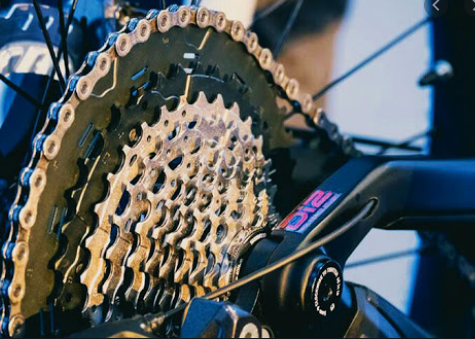
\includegraphics[width=1.8in]{coppiaAlta.png}
  	\caption{That's the caption}
   	\label{fig:picture}
\end{figure}

\subsection{English, please}\label{SPar:unAcc}

another picture


\begin{figure}[h!]		
	\centering
   	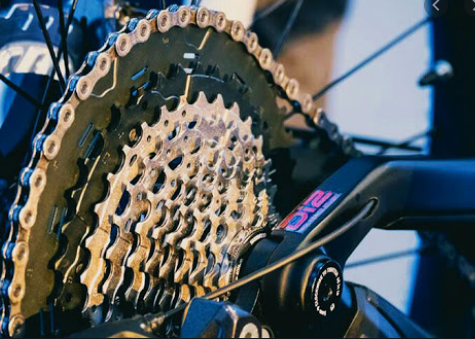
\includegraphics[width=1.8in]{coppiaAlta.png}%
  	\caption{English, please}
   	\label{fig:graficoST_unAcce}
\end{figure}

some words here and there



\section{another section}

one more time a list:

\begin{itemize}
	\item Number 1
	\item Number 2
	\item Number 3
\end{itemize}





\subsection{Another section}

I

\clearpage










\section{Here a section}

in which an equation is written

\begin{eqnarray}
	B_2(t) = \frac{\mu_0\mu_r i_1(t)N_1}{l}\propto V_1(t)
\end{eqnarray}

not only one

\begin{eqnarray}
	\frac{V_1}{V_2} = \frac{N_1}{N_2}
\end{eqnarray}

Ove




\begin{itemize}
	\item $V_1$ \'e la tensione applicata al solenoide primario
	\item $V_2$ \'e la tensione applicata al solenoide secondario
	\item $N_1$ \'e il numero di spire presenti sul solenoide primario
	\item $N_2$ \'e il numero di spire presenti sul solenoide secondario
\end{itemize}

	


\section{Another section}\label{par:OndaMeccanica}


From time to time clearing a page is good


\clearpage

\section{Another section}


\clearpage

\section{Last section, hopefully}\label{cap:elettromagnetiche}

I don't know why, but each time a section is opened a "clearpage" command is provided behind






\end{document}